% Baseado em bare_conf.tex

\documentclass[conference]{IEEEtran}
\usepackage[utf8]{inputenc}
\usepackage[T1]{fontenc}
\usepackage[pdftex]{graphicx}
\usepackage{float}
\usepackage{color}
\usepackage{url}
\IEEEoverridecommandlockouts



% *** SPECIALIZED LIST PACKAGES ***
%
%\usepackage{algorithmic}
% algorithmic.sty was written by Peter Williams and Rogerio Brito.
% This package provides an algorithmic environment fo describing algorithms.
% You can use the algorithmic environment in-text or within a figure
% environment to provide for a floating algorithm. Do NOT use the algorithm
% floating environment provided by algorithm.sty (by the same authors) or
% algorithm2e.sty (by Christophe Fiorio) as IEEE does not use dedicated
% algorithm float types and packages that provide these will not provide
% correct IEEE style captions. The latest version and documentation of
% algorithmic.sty can be obtained at:
% http://www.ctan.org/tex-archive/macros/latex/contrib/algorithms/
% There is also a support site at:
% http://algorithms.berlios.de/index.html
% Also of interest may be the (relatively newer and more customizable)
% algorithmicx.sty package by Szasz Janos:
% http://www.ctan.org/tex-archive/macros/latex/contrib/algorithmicx/

% correct bad hyphenation here
%\hyphenation{op-tical net-works semi-conduc-tor}


\begin{document}
\title{Trekking/Robo-Magellan Project}

\author{\IEEEauthorblockN{ThundeRatz Robotics Team}
\IEEEauthorblockA{Escola Politécnica da\\
Universidade de São Paulo \\
contato@thunderatz.org}
}

\maketitle

\section{Introduction}
\subsection{The team}
Founded in 2001 by a group of engineering undergraduate students from University
of São Paulo (USP) to bring the international robot combat competition to Brazil,
the team does research and development on robotics in the biggest university in
South America. Throughout the years, it expanded into more categories and
competitions, with highlight on its internationally awarded sumo robots
~\cite{All Japan Robot Sumo} and Robo-Magellan~\cite{SRS}. After over 10 years
of experience, learning and university research, the ThundeRatz team~\cite{ThundeRatz}
has some of the most known and award-winning robots of Brazil, reason of pride to
the members and motivation for more innovations.

\subsection{The project}
Trekking~\cite{Trekking} and Robo-Magellan are two competition categories
involving autonomous robots emphasizing navigation and obstacle avoidance over
varied, outdoor terrain. Their goals are autonomous movement and localization.
Both are explained in detail later.

\section{Goals}
\setcounter{section}{0}
The team's main goal is the dissemination of knowledge between its members and
the advancement of robotics nationally through innovations and research. To this
end, the project follows some guidelines:
\subsubsection{Open-source}
Code from past competition editions is open-source and published at the team's
GitHub page ~\cite{Git-TR}.
\subsubsection{Affordable}
Initial versions of the project used a Raspberry Pi, USB camera, compass and
GPS, building a cheap but competitive robot. We are investing in more advanced
technologies to keep the project up-to-date with international competitions, but
most of its concepts can be implemented without a high cost.
\subsubsection{Shared knowledge}
Lots of knowledge and experiences are shared in the competitions and a warm
friendship environment is kept with other teams. Furthermore, the robot is
shown in philanthropic events and expositions.

\medskip
The goals currently set for the project are:
\setcounter{subsection}{0}
\subsection{Increased reliability} Use sensor redundancy and sensor fusion
algorithms~\cite{kalman} to enhance reliability under bad conditions.
\subsection{CUDA-based Computer Vision} Port the already developed knowledge of
computer vision using OpenCV to CUDA.
\subsection{SLAM research} Try to use laser based SLAM techniques for
location and evaluate different SLAM algorithms. Existent laser SLAM CUDA
solutions are mostly under development~\cite{CUDA-PHDSLAM}, but some are complete
~\cite{rgbdslam_v2} and papers and other universities' research are available
~\cite{CUDA-IEEE}. If possible, use existing or create CUDA solutions based on current
research.

\section{Competitions}
\setcounter{subsection}{0}
Competitions create a friendly environment to share ideas and experiences with
other teams and evaluate the project's advancement. The robot takes part in two
similar autonomous categories.
\subsection{Trekking}
Trekking is a national category hosted at the Winter Challenge and Summer
Challenge competitions. Both are hosted by RoboCore~\cite{RoboCore}, a company
specialized in robotics, and are our main competitions. The Trekking category's
goal is the construction of a robot to locate white boards on an open grass field.
The boards can be optionally marked with an orange traffic cone.
\subsection{Robo-Magellan}
Robo-Magellan is an international category held by the Seattle Robotics Society
(SRS)~\cite{SRS}. An autonomous robot is assigned to locate orange traffic cones
hidden in an environment with obstacles. There is no straight-line path between
the start and destination points without some significant obstacle. The robot
must locate and touch as many cones as possible.

\section{Project details}
\setcounter{subsection}{0}
We strive to maintain a competitive and evolving project. Project achievements
can be seen at section~\ref{past-achievements}.
\subsection{First iteration}
The first version of the robot used a compass, GPS and USB camera. It's four
wheel layout with traction on all wheels was kept in later versions, although
the chain transmission was changed. OpenCV was used for computer vision. A
Raspberry Pi was used for processing and a router was included for wireless
programming and debugging.

\begin{figure}[H]
    \centering
    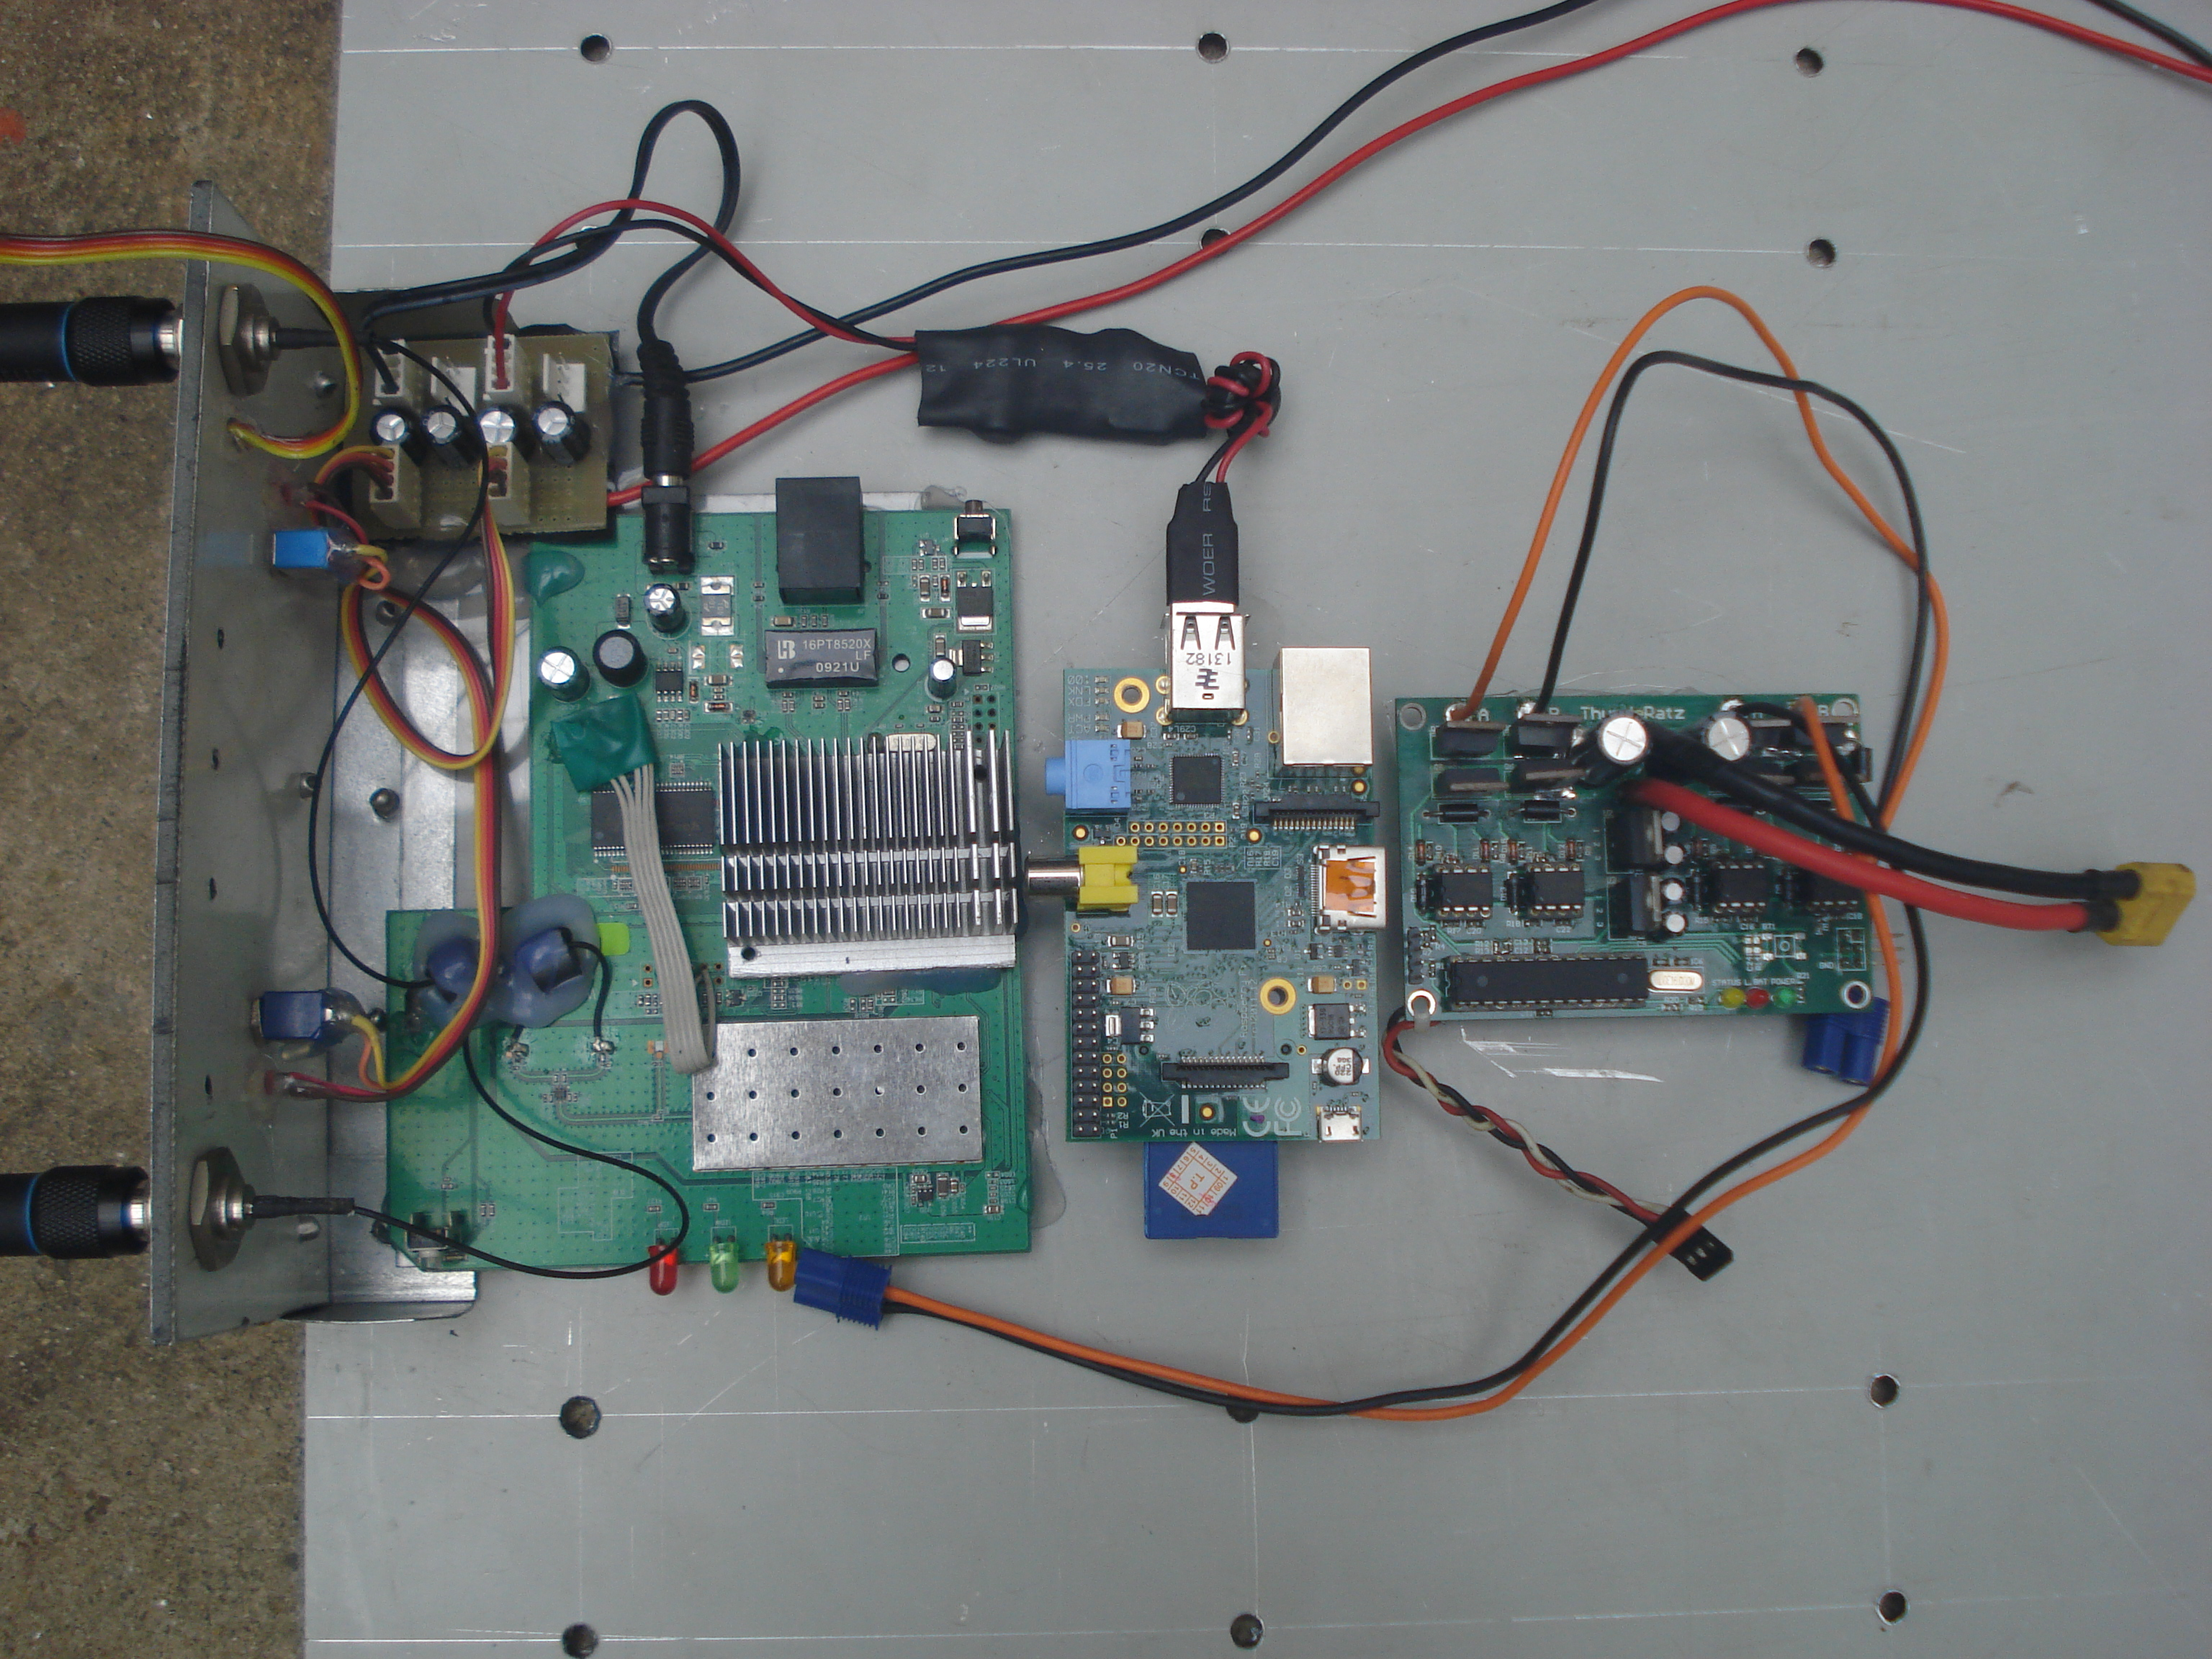
\includegraphics[width=0.45\textwidth]{../Pictures/v1/WCX2014/DSC01671.JPG}
    \caption{Disassembly with electronics exposed. From left to right: router,
    Raspberry Pi B, motor controller}
\end{figure}

\begin{figure}[H]
    \centering
    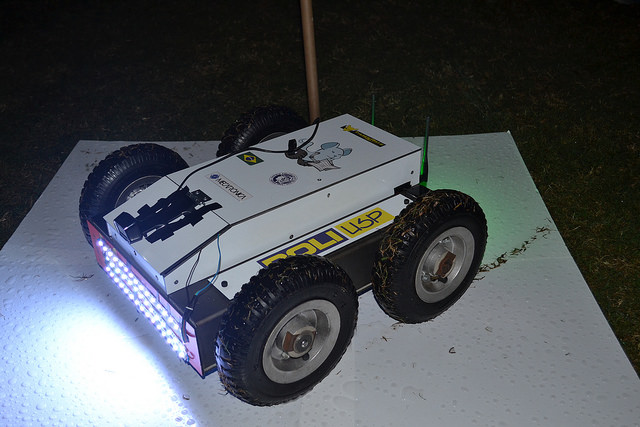
\includegraphics[width=0.45\textwidth]{../Pictures/v1/WCX2014/14749170673_6e4bfca9fc_z.jpg}
    \caption{Robot at Winter Challenge X (São Paulo, Brazil), 2014}
\end{figure}

\begin{figure}[H]
    \centering
    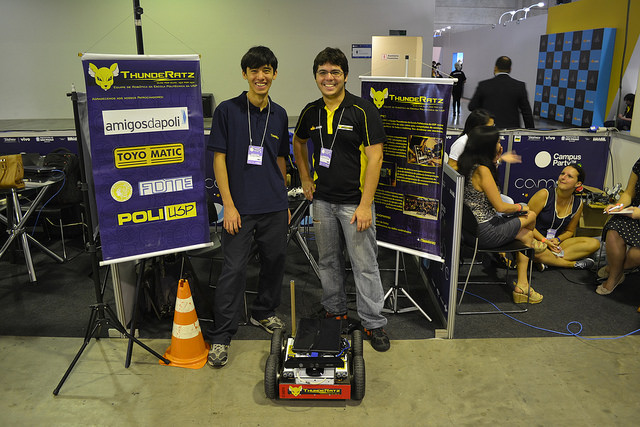
\includegraphics[width=0.45\textwidth]{../Pictures/v1/URC2014/16907969931_064dda21f8_z.jpg}
    \caption{Robot at Campus Future (Campus Party 2015)~\cite{Campus-Future},
    open exposition of new engineering projects}
\end{figure}

\subsection{Second iteration}
The robot went through changes to compete on the Robo-Magellan category.
The weight limitation, which doesn't exist on the Trekking category, required
a lighter structure. We also used faster motors.
The USB camera was replaced by a CMUCam 5, camera with integrated image
processing and color detection. HC-SR04 sonars were added to detect the
distance to the traffic cones.
It was its first international competition and the team's first time at the
United States.

\begin{figure}[H]
    \centering
    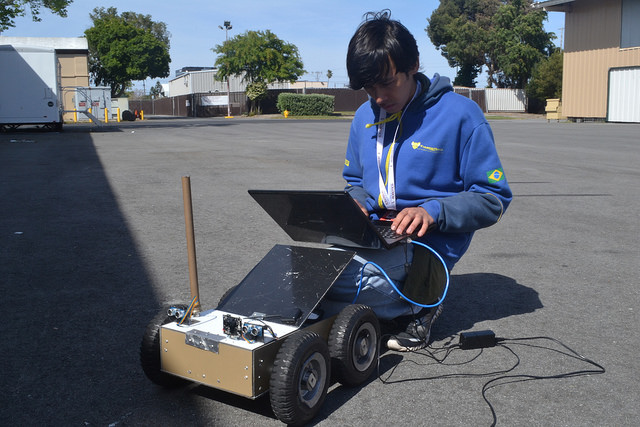
\includegraphics[width=0.45\textwidth]{../Pictures/v2/RG2015/16982466210_3565d58788_z.jpg}
    \caption{RoboGames 2015 (San Mateo, CA)}
\end{figure}

\begin{figure}[H]
    \centering
    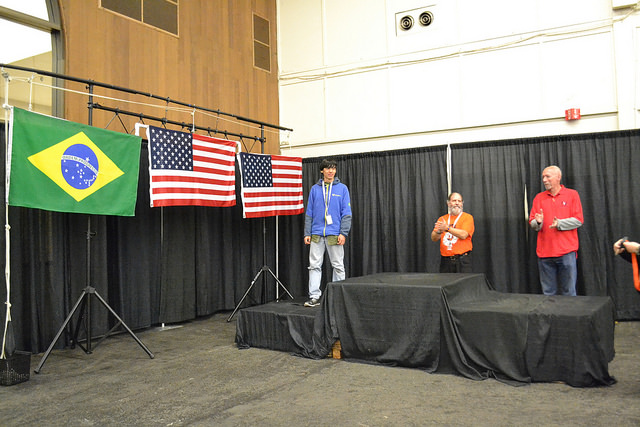
\includegraphics[width=0.45\textwidth]{../Pictures/v2/RG2015/17168959772_304585a0eb_z.jpg}
    \caption{Third place at RoboGames 2015}
\end{figure}

\subsection{Third iteration}
The third iteration is the current project. Smaller and lighter, its goal is to
create a robust project, with sensor redundancy and new sensing technologies.
It currently uses a Raspberry Pi B 2.0 as its main computer. One of our goals is
to make embedded computer vision and learning and SLAM possible in the project.
To reach them real time in an embedded platform, GPU acceleration will be required.
The robot was used in Winter Challenge XI, but due to problems in our electronics
it got 5th place. It was also used in Summer Challenge III, achieving 2nd place, RoboGames 2016 on 3rd and Winter Challenge XII on 4th. 

\begin{figure}[H]
    \centering
    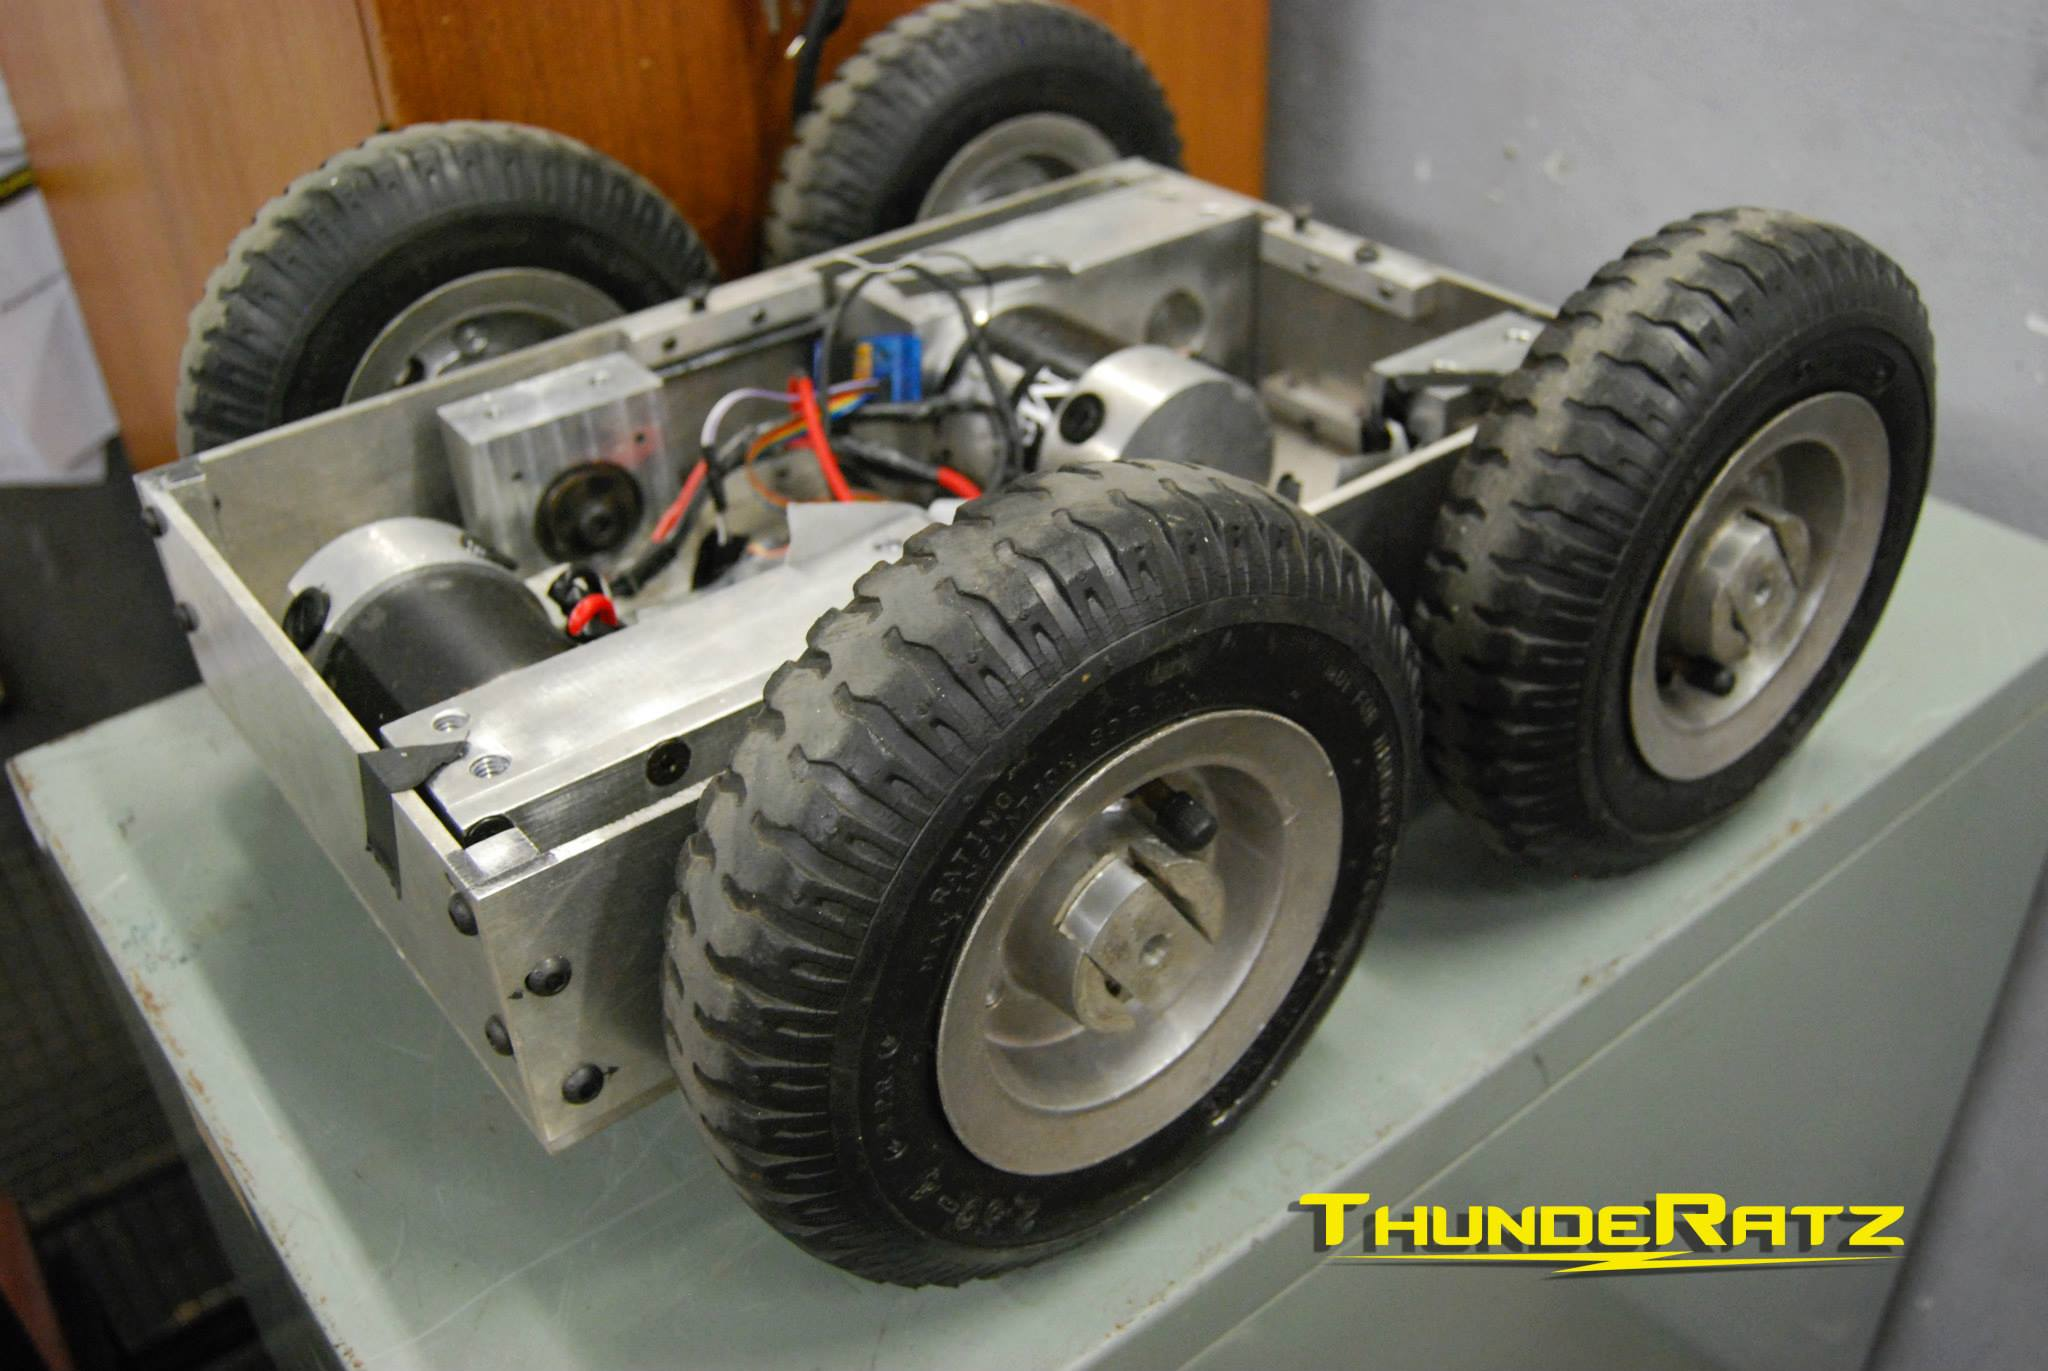
\includegraphics[width=0.45\textwidth]{../Pictures/v3/WCXI2015/1404454_850450764990318_6911866873946202760_o.jpg}
    \caption{Robot structure}
\end{figure}

\begin{figure}[H]
    \centering
    \includegraphics[width=0.45\textwidth]{../Pictures/v3/WCXI2015/DSC01916.JPG}
    \caption{Raspberry Pi B 2.0 with team-made GPS module}
\end{figure}

\begin{figure}[H]
    \centering
    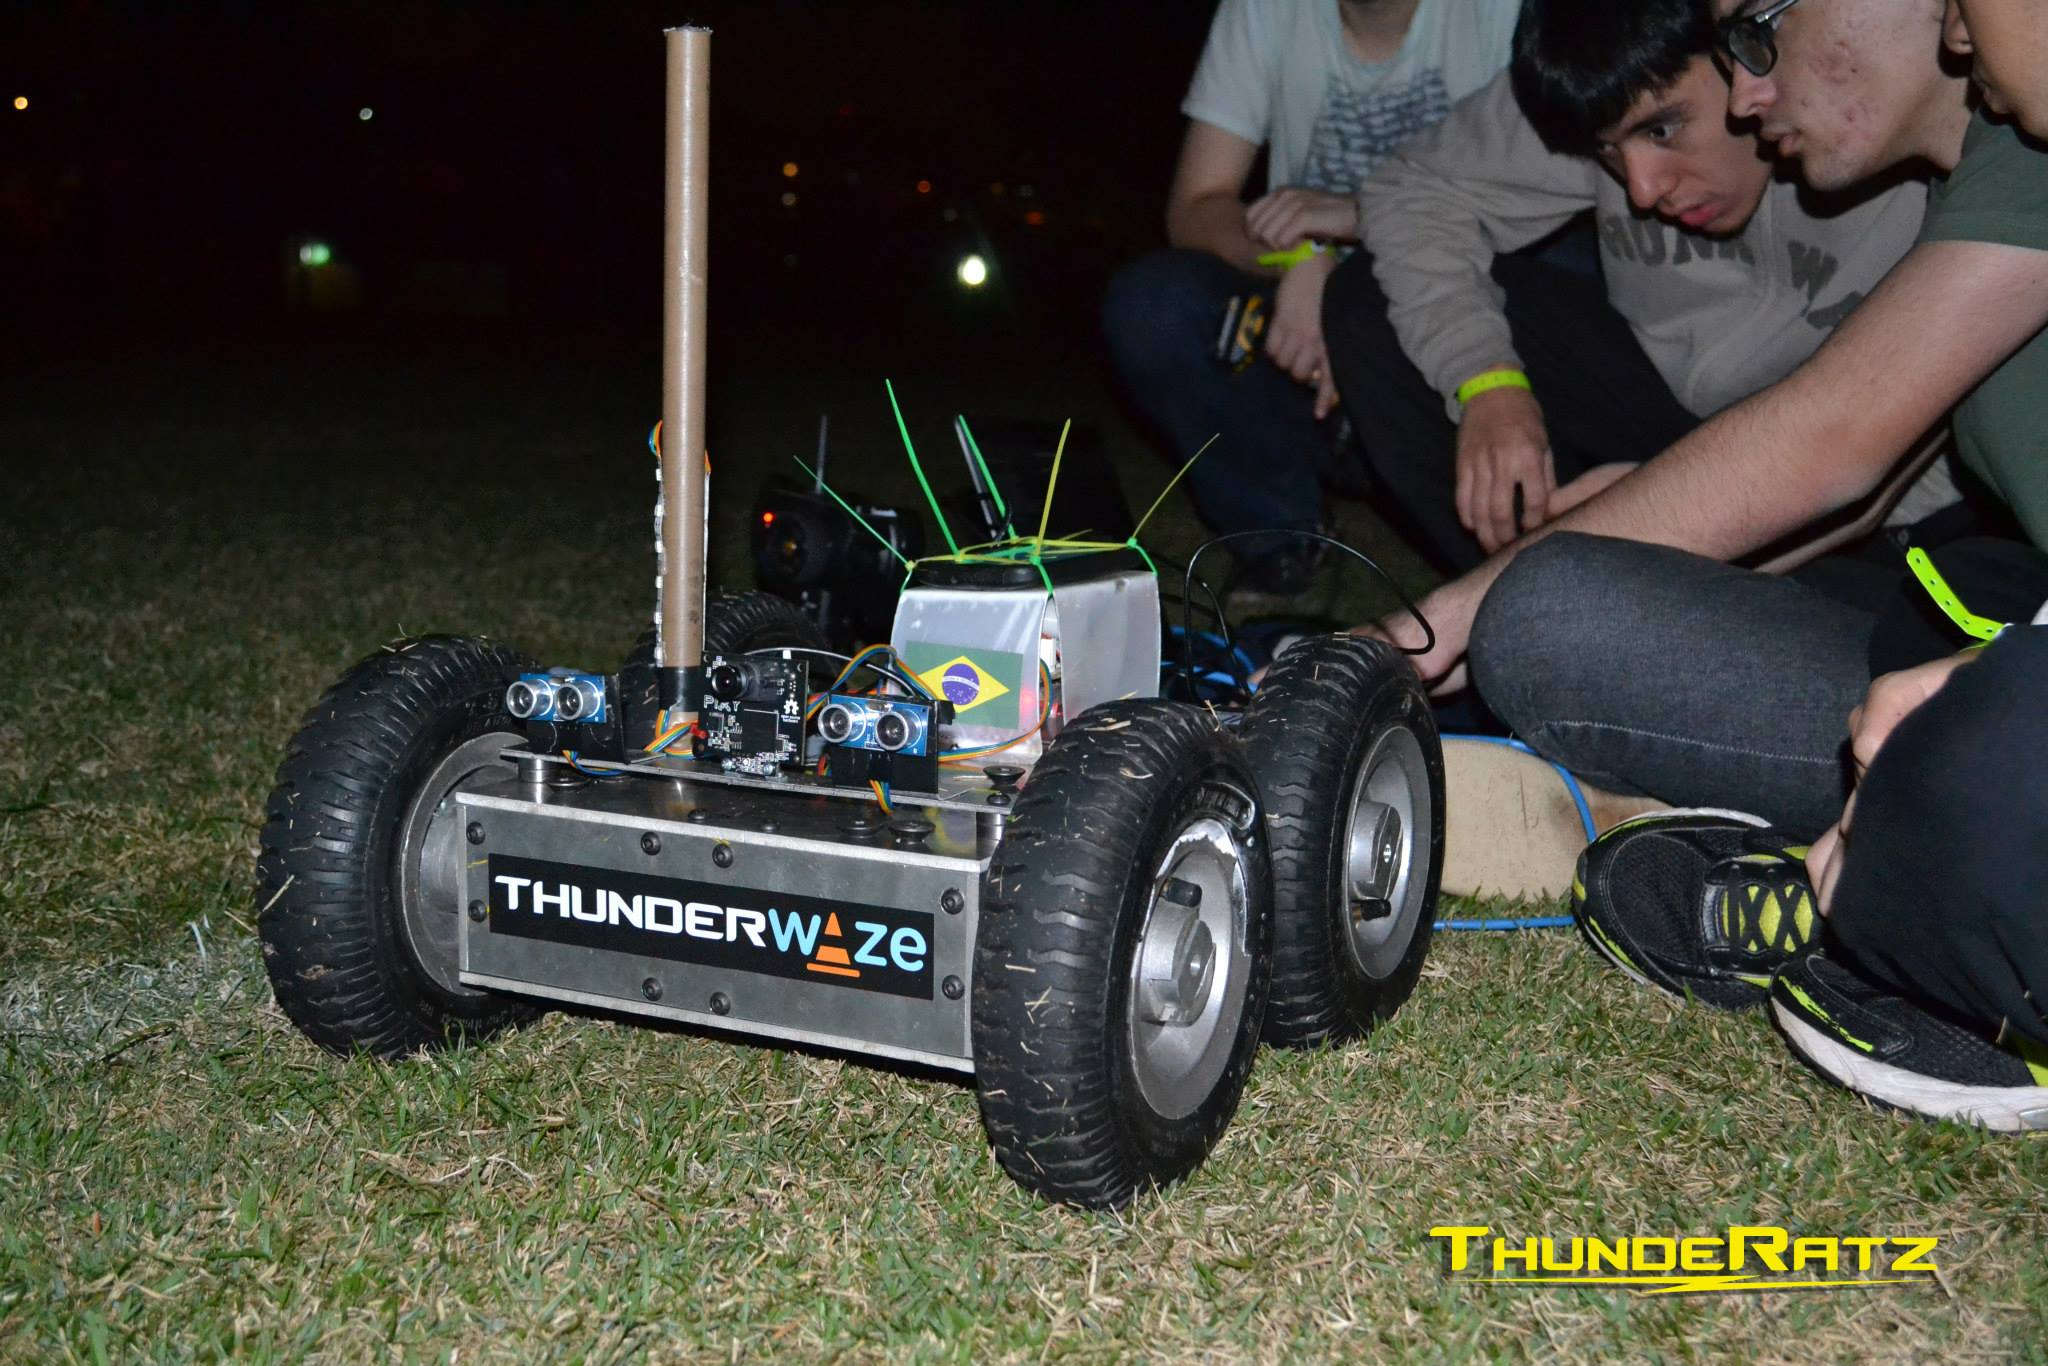
\includegraphics[width=0.45\textwidth]{../Pictures/v3/WCXI2015/11402892_850967411605320_3887305866160117339_o.jpg}
    \caption{Winter Challenge XI (São Paulo, Brazil), 2015}
\end{figure}

% Colocar imagem do Summer aqui
%\begin{figure}[H]
%    \centering
%    \includegraphics[width=0.45\textwidth]{../Pictures/v3/SCIII2015/[Imagem aqui].jpg}
%    \caption{Summer Challenge III (Minas Gerais, Brazil), 2015}
%\end{figure}


\subsection{Fourth iteration}
This project is currently intended on being remastered once more. Now optimized in space, its goal is to go for full capability of the provided hardware. Now with more sensors and new interpretation technologies.
It currently uses a Nvidia TK1 as its main computer. One of our goals is
to make object identification through machine-learning in the project.
To develop the neural network systems capable of machine-learning, systems with support for Digits will be required.

\section{Past achievements} \label{past-achievements}
Our robot is one of the national favorites and proudly the international
third place. Being a reasonably recent project, it hasn't gone through a lot of
competitions. Following is a list of past achievements.

\subsection*{2014}
\setcounter{subsubsection}{0}
\subsubsection{Winter Challenge X} Third place
\subsection*{2015}
\setcounter{subsubsection}{0}
\subsubsection{RoboGames 2015} Third place
\subsubsection{Winter Challenge XI} Fifth place
\subsubsection{Summer Challenge III} Second place
\subsection*{2016}
\setcounter{subsubsection}{0}
\subsubsection{RoboGames 2016} Third place
\subsubsection{Winter Challenge XII} Fourth place

\section{Partnership}
Companies willing to help the project are encouraging university research and
knowledge dissemination. Partner companies get their logo on the robot and team's
t-shirts, which are worn by the team's members in competitions, expositions
and in daily activities in the university.

\section*{Acknowledgment}
We gratefully acknowledge the support of LeddarTech with the donation of the
Leddar Sensor Evaluation Kit and NVIDIA Corporation with the donation of
the Jetson TK1 GPU used for this project.

\begin{thebibliography}{30}
    \bibitem{All Japan Robot Sumo}
    FSI-All Japan Robot-Sumo Tournament. \emph{Robot Sumo Overview}. http://www.fsi.co.jp/sumo-e/out/out00000.html
    \bibitem{SRS}
    Seattle Robotics Society. \emph{SRS Robo-Magellan}. http://www.robothon.org/robothon/robo-magellan.php
    \bibitem{ThundeRatz}
    ThundeRatz Robotics Team. http://thunderatz.org/
    \bibitem{Trekking}
    RoboCore. \emph{Trekking rules}. \url{https://www.robocore.net/upload/attachments/robocore__regras_robo_trekking_976.pdf}
    \bibitem{Git-TR}
    GitHub. \emph{Thunderatz Robotics Team} https://github.com/ThundeRatz
    \bibitem{kalman}
    SourceForge. \emph{KFilter}. http://kalman.sourceforge.net/
    \bibitem{CUDA-PHDSLAM}
    Chee Sing Lee. \emph{PHD Filter SLAM with CUDA} https://github.com/cheesinglee/cuda-PHDSLAM
    \bibitem{rgbdslam_v2}
    Felix Endres. \emph{Rgbdslam v2} \url{http://felixendres.github.io/rgbdslam_v2/}
    \bibitem{CUDA-IEEE}
    Haiyang Zhang, Fred Martin. \emph{CUDA Accelerated Robot Localization and Mapping}
    http://ieeexplore.ieee.org/stamp/stamp.jsp?arnumber=6556350
    \bibitem{RoboCore}
    RoboCore. \emph{Sua tecnologia à prova}. https://www.robocore.net/
    \bibitem{Campus-Future}
    Campus Party. \emph{Campus Future}. http://brasil.campus-party.org/conteudos/open-campus/campus-future/
\end{thebibliography}

\end{document}

% An example of a floating figure using the graphicx package.
% Note that \label must occur AFTER (or within) \caption.
% For figures, \caption should occur after the \includegraphics.
% Note that IEEEtran v1.7 and later has special internal code that
% is designed to preserve the operation of \label within \caption
% even when the captionsoff option is in effect. However, because
% of issues like this, it may be the safest practice to put all your
% \label just after \caption rather than within \caption{}.
%
% Reminder: the "draftcls" or "draftclsnofoot", not "draft", class
% option should be used if it is desired that the figures are to be
% displayed while in draft mode.
%
%\begin{figure}[!t]
%\centering
%\includegraphics[width=2.5in]{myfigure}
% where an .eps filename suffix will be assumed under latex,
% and a .pdf suffix will be assumed for pdflatex; or what has been declared
% via \DeclareGraphicsExtensions.
%\caption{Simulation results for the network.}
%\label{fig_sim}
%\end{figure}

% Note that IEEE typically puts floats only at the top, even when this
% results in a large percentage of a column being occupied by floats.


% An example of a double column floating figure using two subfigures.
% (The subfig.sty package must be loaded for this to work.)
% The subfigure \label commands are set within each subfloat command,
% and the \label for the overall figure must come after \caption.
% \hfil is used as a separator to get equal spacing.
% Watch out that the combined width of all the subfigures on a
% line do not exceed the text width or a line break will occur.
%
%\begin{figure*}[!t]
%\centering
%\subfloat[Case I]{\includegraphics[width=2.5in]{box}%
%\label{fig_first_case}}
%\hfil
%\subfloat[Case II]{\includegraphics[width=2.5in]{box}%
%\label{fig_second_case}}
%\caption{Simulation results for the network.}
%\label{fig_sim}
%\end{figure*}
%
% Note that often IEEE papers with subfigures do not employ subfigure
% captions (using the optional argument to \subfloat[]), but instead will
% reference/describe all of them (a), (b), etc., within the main caption.
% Be aware that for subfig.sty to generate the (a), (b), etc., subfigure
% labels, the optional argument to \subfloat must be present. If a
% subcaption is not desired, just leave its contents blank,
% e.g., \subfloat[].


% An example of a floating table. Note that, for IEEE style tables, the
% \caption command should come BEFORE the table and, given that table
% captions serve much like titles, are usually capitalized except for words
% such as a, an, and, as, at, but, by, for, in, nor, of, on, or, the, to
% and up, which are usually not capitalized unless they are the first or
% last word of the caption. Table text will default to \footnotesize as
% IEEE normally uses this smaller font for tables.
% The \label must come after \caption as always.
%
%\begin{table}[!t]
%% increase table row spacing, adjust to taste
%\renewcommand{\arraystretch}{1.3}
% if using array.sty, it might be a good idea to tweak the value of
% \extrarowheight as needed to properly center the text within the cells
%\caption{An Example of a Table}
%\label{table_example}
%\centering
%% Some packages, such as MDW tools, offer better commands for making tables
%% than the plain LaTeX2e tabular which is used here.
%\begin{tabular}{|c||c|}
%\hline
%One & Two\\
%\hline
%Three & Four\\
%\hline
%\end{tabular}
%\end{table}


% Note that the IEEE does not put floats in the very first column
% - or typically anywhere on the first page for that matter. Also,
% in-text middle ("here") positioning is typically not used, but it
% is allowed and encouraged for Computer Society conferences (but
% not Computer Society journals). Most IEEE journals/conferences use
% top floats exclusively.
% Note that, LaTeX2e, unlike IEEE journals/conferences, places
% footnotes above bottom floats. This can be corrected via the
% \fnbelowfloat command of the stfloats package.
